\newlength\colwidth
\newlength\topstripheight
\setlength{\colwidth}{.49\textwidth}
\setlength{\topstripheight}{.4\textheight}
% -----------------------------------------------------------------------
\hbox to \textwidth{%
\tbox{%
% ---------------------------------------------------
% Left side: Intro
% ---------------------------------------------------
\begin{minipage}[t]{\colwidth}%
\vskip 0pt%
% ---------------------------------------------------
\begin{figure}[tb]
\def\PicWidth{0.24\textwidth}%
\centering%
\begin{subfigure}[b]{\PicWidth}
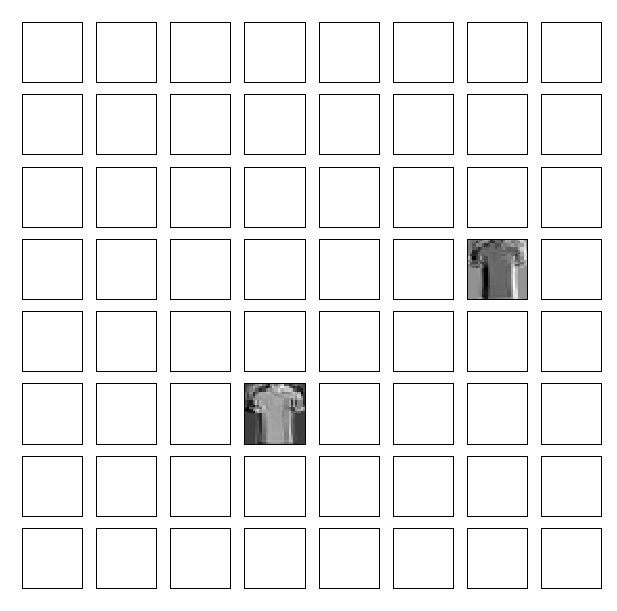
\includegraphics[width=\textwidth,trim=0.35cm 0.35cm 0.2cm 0.35cm,clip]{atelier/FMNIST/FM_e0.pdf}%
\caption{Iteration 0}
\end{subfigure}
\hfill%
%
\begin{subfigure}[b]{\PicWidth}
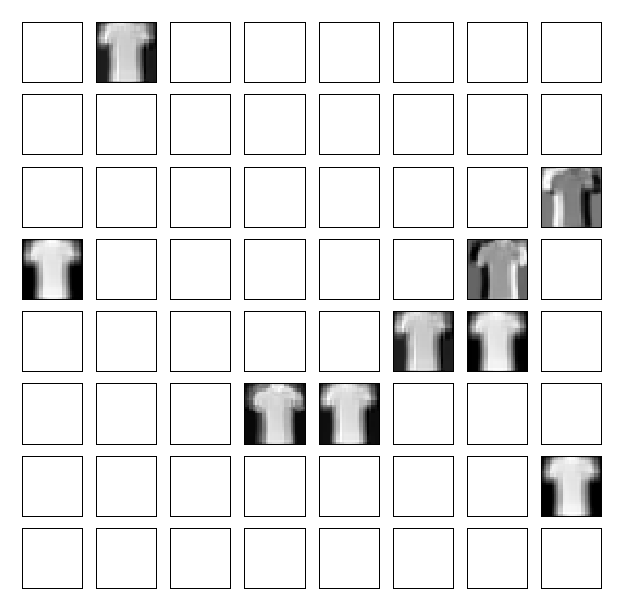
\includegraphics[width=\textwidth,trim=0.35cm 0.35cm 0.2cm 0.35cm,clip]{atelier/FMNIST/FM_e5.pdf}%
\caption{Iteration 5}
\end{subfigure}
\hfill%
%
\begin{subfigure}[b]{\PicWidth}
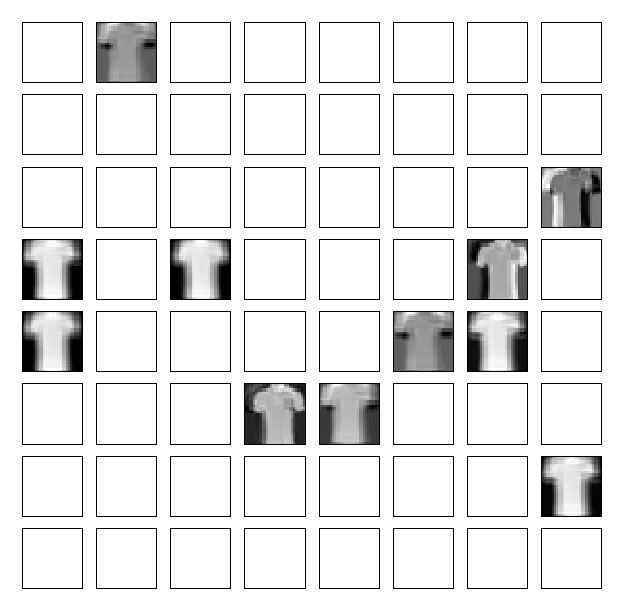
\includegraphics[width=\textwidth,trim=0.35cm 0.35cm 0.2cm 0.35cm,clip]{atelier/FMNIST/FM_e20.pdf}%
\caption{Iteration 20}
\end{subfigure}
\hfill%
%
\begin{subfigure}[b]{\PicWidth}
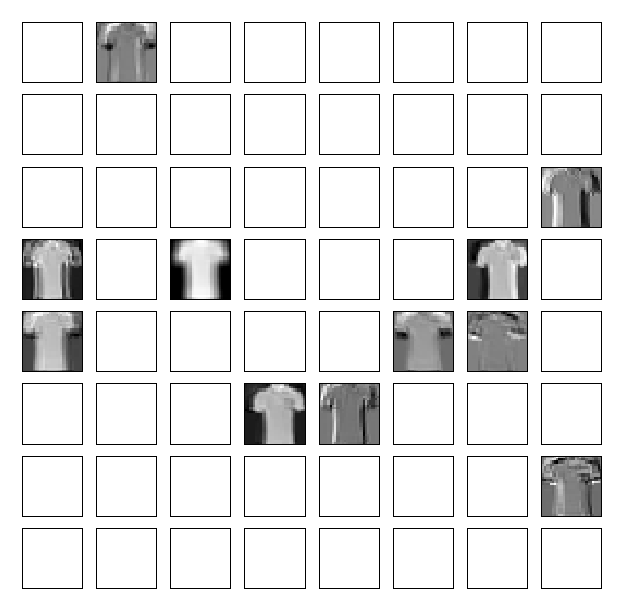
\includegraphics[width=\textwidth,trim=0.35cm 0.35cm 0.2cm 0.35cm,clip]{atelier/FMNIST/FM_e100.pdf}%
\caption{Iteration 100}
\end{subfigure}
\caption{Inverse scale space character of \LinBreg{} \cite{Bungert22} visualized through feature maps of a convolutional neural network. Active kernels are added in the training process.}
\label{fig:kernels}
\vspace{-10pt}
\end{figure}
% ---------------------------------------------------
%
%
%
%
\vspace{1cm}%

\cblock{BaseColor}{}{Bregman Training in a Nutshell}{%
\footnotesize%
\vspace{.1em}%

For input and output spaces $\Inp, \Oup$ we denote by $\net_\param:\Inp\to\Oup$ a neural network parameterized by $\param$ from some parameter space $\Param$. For a feed-forward have that $\net_\param = \Phi^L\circ\ldots\circ\Phi^1$ where the $l$-th layer is given by
%
\begin{align*}
\Phi^L: x\mapsto \sigma\left(W^l x + b^l\right).
\end{align*}
Here, $W^l, b^l$ denote the weights and biases of the $l$-th layer and $\sigma$ is an activation function.
}
\vspace{.5em}

%
\begin{minipage}[t]{.48\textwidth}%
\vskip0pt%
\begin{itemize}%
\small%
\item We want to minimize some loss \textcolor{BaseDarkColor}{\textbf{loss}} $\empLoss:\Param\to\R$.
\item Employing batch gradients leads to a \textcolor{BaseDarkColor}{\textbf{stochastic}} version of Bregman Iterations \cite{yin2008bregman}.
\end{itemize}
\end{minipage}%
%
\hfill%
%
\begin{minipage}[t]{.48\textwidth}%
\vskip0pt%
\begin{itemize}%
\small%
\item We want to enforce \textcolor{BaseDarkColor}{\textbf{sparsity}}.
\item This is done via an \textcolor{BaseDarkColor}{\textbf{regularization}} functional $\func:\Param\to\R$, e.g.,
%
\begin{align*}
\func(\param) &= \sum_{l=1}^L \norm{W^l}_{1,1}.
\end{align*}
\end{itemize}%
\end{minipage}%
\vspace{1cm}

%
\begin{minipage}[t]{\textwidth}%
\cblock{BaseColor}{}{The Algorithm\phantom{C}}{%
\begin{itemize}
\small%
\item Initialize sparse parameters $\theta^{(0)}$ and $v^{(0)}\in\partial J(\theta^{(0)})$.
\item Denote by $g:\Param\times\Omega \to \Param$ an unbiased estimator of $\nabla\empLoss$ for some probability space $(\Omega, \P)$, sample $\omega^{(k)}$ according to $\P$ and set $g^{(k)} = g(\theta^{(k)}; \omega^{(k)})$.
\end{itemize}%

\begin{minipage}[t]{.3\textwidth}%
\vskip0pt%
\normalsize%
\colorlet{FAUBlueA}{FAUBlue!62.5}
\setbeamercolor{hcolor}{fg=white,bg=BaseColorB}%
\begin{beamercolorbox}[wd=\textwidth, ht=3.5cm, sep=0pt,dp=0pt,center]{hcolor}%
\vbox to 3.5cm{%
\vfill%
LinBreg Update
\vfill%
}%
\end{beamercolorbox}%
\end{minipage}%
%
\begin{minipage}[t]{.7\textwidth}%
\vskip0pt%
\normalsize%
\setbeamercolor{hcolor}{fg=black,bg=BaseColorD}%
\begin{beamercolorbox}[wd=\textwidth, ht=3.5cm, sep=0pt,dp=0pt]{hcolor}%
\begin{align*}%
v^{(k+1)} &:= v^{(k)} - \tau^{(k)} g^{(k)},\qquad&\text{Gradient Step}\\
\param^{(k+1)} &:= \prox{\delta J}(\delta v^{(k+1)}).
\qquad&\text{Proximal Step}
\end{align*}%
\end{beamercolorbox}%
\end{minipage}%
}%
\end{minipage}%
\end{minipage}%
}%
%
%
%
%
% ---------------------------------------------------
% Line Divider
% ---------------------------------------------------
\hfill%
%
\tbox{%
\begin{minipage}[t]{.005\textwidth}%
\vskip 0pt%
\begin{center}
\textcolor{BaseColor}{%
\rule{.2mm}{\topstripheight}%
}
\end{center}
\end{minipage}%
}%
%
\hfill%
%
%
%
%
%
% ---------------------------------------------------
% Analytical Results
% ---------------------------------------------------
\tbox{%
\begin{minipage}[t]{\colwidth}%
\vskip 0pt%
%
%
\cblock{BaseColor}{}{Background and Assumptions}{}%
%Section for assumptions
\begin{minipage}{\textwidth}%
\small%
The Bregman distance of two points $\param,\overline{\param}\in\Param$ with respect to a convex and proper functional $\func:\Param\to(-\infty,\infty]$ is given as
%
\begin{align*}
D^\sg_\func(\overline{\param},\param) := \func(\overline \param)-\func({\param})-\langle\sg,\overline\param-{\param}\rangle,\quad\sg\in\partial\func(\param).
\end{align*}
%
\vspace{.2em}

\begin{minipage}[t]{.48\textwidth}%
\footnotesize%
\textbf{Assumption 1: The Loss function}

We assume that $\empLoss\geq 0$, $\empLoss$ is continuously differentiable and that for all $\param,\tilde\param\in\Param$ we have
\begin{align*}
\norm{\nabla\empLoss(\tilde\param)-\nabla\empLoss(\param)}\leq L \norm{\tilde\param-\param}.
\end{align*}%
\end{minipage}%
%
\hfill
%
\begin{minipage}[t]{.48\textwidth}%
\footnotesize%
\textbf{Assumption 2: Bounded Variance}


There exists a constant $\sigma>0$ such that for any $\param\in\Param$ it holds
\begin{align*}
\E\left[\norm{g(\param;\cdot)-\nabla\empLoss(\param)}^2\right] \leq \sigma^2.
\end{align*}%
\end{minipage}%
\end{minipage}%
%
\vspace{.5em}

%
\begin{minipage}{\textwidth}%
\small%
\begin{minipage}[t]{.48\textwidth}%
\footnotesize%
\textbf{Assumption 3: Regularizer}

We assume that $\func:\Param\to(-\infty,\infty]$ is a convex, proper, and lower semicontinuous functional on the Hilbert space $\Param$.%
\end{minipage}%
%
\hfill%
%
\begin{minipage}[t]{.48\textwidth}%
\footnotesize%
\textbf{Assumption 4: Strong Convexity}

We have that for all $\param,\tilde\param\in\Param$
\begin{align*}
\empLoss(\tilde\param) &\geq \empLoss(\param) + \langle\nabla\empLoss(\param),\tilde\param - \param\rangle
+ \frac{\mu}{2}\norm{\tilde\param-\param}^2.
\end{align*}%
\end{minipage}%
\end{minipage}%
\vspace{66pt}

%
%
%
%
\cblock{BaseColor}{}{Loss Decay}{%
% section for loss decay
\small
Assume that Assumptions 1--3 hold true, let $\delta>0$, then there exist constants $c,C>0$ such that for every $k\in\N$ the iterates satisfy
\begin{block}{}
\begin{align*}
\textcolor{BaseColor}{\E\left[\empLoss(\param^{(k+1)})\right]} &+
%
\frac{1}{\tau^{(k)}}\E\left[ D^\mathrm{sym}_\func(\param^{(k+1)},\param^{(k)})\right]\\
%
&+
\frac{C}{2\delta\tau^{(k)}}\E\left[\norm{\param^{(k+1)}-\param^{(k)}}^2\right] %\\
%
\leq
\textcolor{BaseColor}{\E\left[\empLoss(\param^{(k)})\right]} + \tau^{(k)}\delta\frac{\sigma^2}{2c}.
\end{align*}
\end{block}
%
\footnotesize%
Here, the step sizes are non-increasing and satisfy $\tau^{(k)} \leq \frac{2}{\delta L}$, $\ell^2 \ni (\tau^{(k)}) \notin \ell^1$.
}%
%
%
%
\vspace{66pt}%

\cblock{BaseColor}{}{Convergence in Norm\phantom{THAh}}{%
\small%
Assume that Assumptions 1--4 hold true and that $J(\param^*)<\infty$, where  $\param^*$ is the unique minimizer of $\mathcal{L}$. For every $k\in\N$ and  $d_k:=\E\left[D_{\func_\delta}^{v^{(k)}}(\param^*,\param^{(k)})\right]$ we have
%
\begin{block}{}
\begin{align*}
d_{k+1} - d_k
+ \frac{\mu}{4}\tau^{(k)}
\E\left[\textcolor{BaseColor}{\norm{\param^*-\param^{(k+1)}}}^2\right]
%
\leq  \frac{\sigma}{2}\left((\tau^{(k)})^2 +\Exp{\norm{\param^{(k)} - \param^{(k+1)}}^2}\right).
\end{align*}
\end{block}
%
Furthermore, there exists a subsequence $\param^{(k_j)}$ such that
\begin{align*}
\lim_{j\to\infty}\E\left[\norm{\param^*-\param^{(k_j)}}^2\right] = 0.
\end{align*}
}%
\end{minipage}%
}%
}



